\begin{table*}[t]
  \captionof{table}{Connection vs Assignment}
  \label{tbl:Box}
  \begin{tabular}{|c|c|c|}
    \hline 
    \textbf{Criteria} & \textbf{Connection} & \textbf{Assignment} \\ 
    \hline
    \begin{minipage}{0.1\textwidth}
      \flushleft
      Code
    \end{minipage} 
    &
    \begin{minipage}[c][1.7cm]{0.4\textwidth}
      \begin{minted}[autogobble,tabsize=2,framesep=1pt,fontfamily=pcr,fontsize=\fontsize{8}{9}\selectfont]{scala}
      trait IOConnection extends DFDesign {
        val i = DFUInt[8] <> IN
        val o = DFUInt[8] <> OUT
        o <> i
      }
      \end{minted}
    \end{minipage} 
    &  
    \begin{minipage}[c][1.7cm]{0.4\textwidth}
      \begin{minted}[autogobble,tabsize=2,framesep=1pt,fontfamily=pcr,fontsize=\fontsize{8}{9}\selectfont]{scala}
        trait IOAssignment extends DFDesign {
          val i = DFUInt[8] <> IN
          val o = DFUInt[8] <> OUT
          o := i
        }
      \end{minted}
    \end{minipage} 
    \\ 
    \hline 
    \begin{minipage}{0.1\textwidth}
      \flushleft
      Functional Diagram
    \end{minipage} 
    &
    \begin{minipage}[c][2.4cm]{0.10\textwidth}
      \centering
      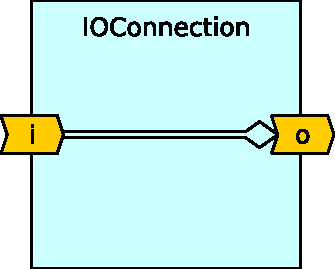
\includegraphics[height=2cm]{graphics/IOConnection.pdf}\\
    \end{minipage}%
    \hfill 
    \begin{minipage}[c][2.4cm]{0.27\textwidth}
      A double line arrow indicates a dataflow dependency \textbf{with} an initial condition dependency.
    \end{minipage} 
    &  
    \begin{minipage}[c][2.4cm]{0.10\textwidth}
      \centering
      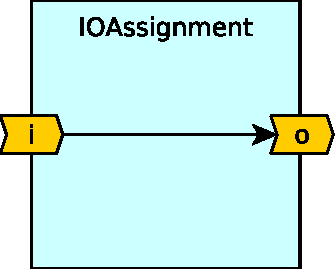
\includegraphics[height=2cm]{graphics/IOAssignment.pdf}\\
    \end{minipage}%
    \hfill 
    \begin{minipage}[c][2.4cm]{0.27\textwidth}
      A single line arrow indicates a dataflow dependency \textbf{without} affecting initial conditions of the consumer.
    \end{minipage} 
    \\ 
    \hline
    \begin{minipage}{0.1\textwidth}
      \flushleft
      Directionality \\and\\ Commutativity
    \end{minipage} 
    &
    \begin{minipage}[c][2cm]{0.42\textwidth}
      The operator is commutative, meaning \code{a <> b} is equivalent to \code{b <> a}. One argument is the \emph{producer}, while the other is the \emph{consumer}. The dataflow direction is sensitive to the context in which the operator is applied.
    \end{minipage} 
    &  
    \begin{minipage}[c][2cm]{0.42\textwidth}
      The operator is non-commutative, meaning \code{a := b} determines that \code{b} is the \emph{producer}, transferring data to the \emph{consumer} \code{a}.
    \end{minipage} 
    \\ 
    \hline
    \begin{minipage}{0.1\textwidth}
      Initialization
    \end{minipage} 
    &
    \begin{minipage}[c][1cm]{0.42\textwidth}
      Initialization is transferred to the consumer.
    \end{minipage} 
    &  
    \begin{minipage}[c][1cm]{0.42\textwidth}
      The consumer initialization is \textbf{not} affected.
    \end{minipage} 
    \\ 
    \hline
    \begin{minipage}{0.1\textwidth}
      \flushleft
      Mutation
    \end{minipage} 
    &
    \begin{minipage}[c][1cm]{0.42\textwidth}
      A consumer can only be connected once at each bit.
    \end{minipage} 
    &  
    \begin{minipage}[c][1cm]{0.42\textwidth}
      The same bit in a consumer can be assigned to 
    \end{minipage} 
    \\ 
    \hline
    \begin{minipage}{0.1\textwidth}
      \flushleft
      Statement Order
    \end{minipage} 
    &
    \begin{minipage}[c][1cm]{0.42\textwidth}
      Connections statements can be placed in any order.
    \end{minipage} 
    &  
    \begin{minipage}[c][1cm]{0.42\textwidth}
      Assignment statements
    \end{minipage} 
    \\ 
    \hline
  \end{tabular}% 
  \vspace{3ex}
  \begin{minipage}[t][9cm][t]{0.34\linewidth}
    \centering
    \captionsetup{justification=centering}    
    \begin{minted}[xleftmargin=1em,linenos,autogobble,tabsize=2,framesep=1pt,frame=single,fontfamily=courier,fontsize=\fontsize{7}{8}\selectfont]{scala}
      trait Box extends DFDesign {
        val iT = DFSInt[16] <> IN
        val iB = DFSInt[16] <> IN
        val oT = DFSInt[16] <> OUT
        val oB = DFSInt[16] <> OUT
        iT.prev <> oT //connection
        oB := iB.prev //assignment
      }
      
      
      
      
      trait BoxTop extends DFDesign {
        val iT = DFSInt[16] <> IN init(5, 7)
        val iB = DFSInt[16] <> IN init(2, 6)
        val oT = DFSInt[16] <> OUT
        val oB = DFSInt[16] <> OUT
        val boxL = new Box {}
        val boxR = new Box {}
        boxL.iT <> iT      
        boxL.iB <> iB
        boxL.oT <> boxR.iT 
        boxL.oB <> boxR.iB
        boxR.oT <> oT      
        boxR.oB <> oB
      }
    \end{minted}
    \vfill
    \captionof{figure}{Bla Bla \\ What we see}
    \label{fig:BoxTopCode}
  \end{minipage}%
  \hfill
  \begin{minipage}[t][9cm][b]{0.64\linewidth}
    \centering
    \captionsetup{justification=centering}
    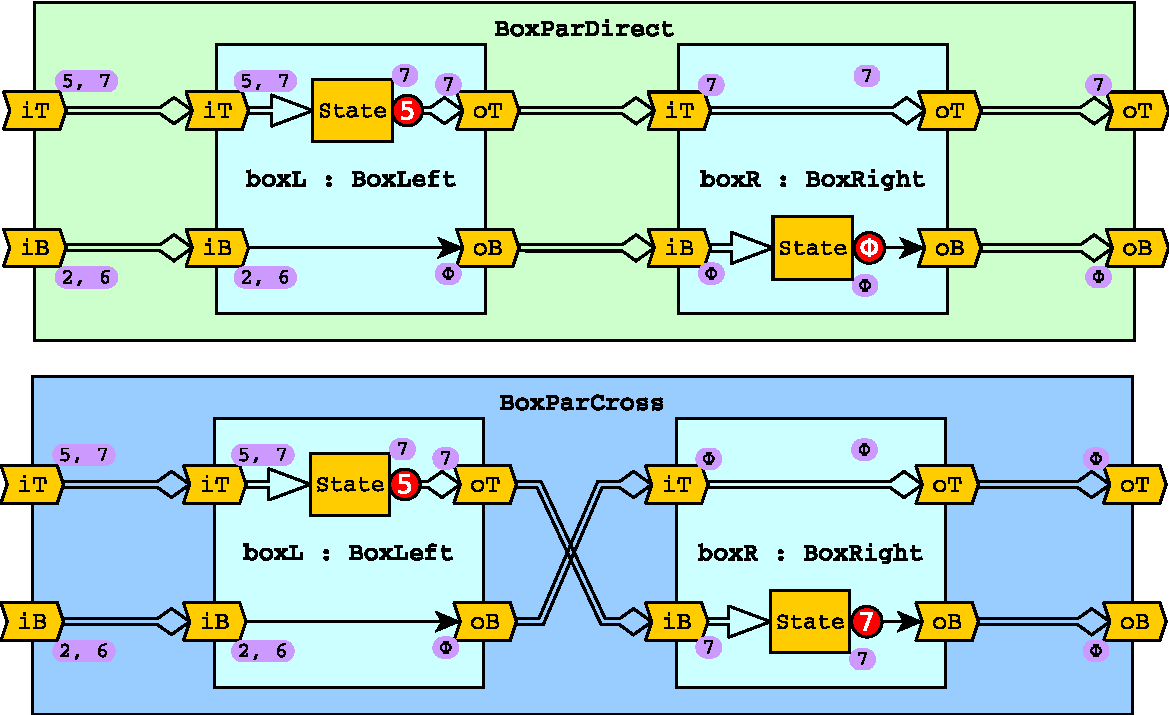
\includegraphics[width=\linewidth]{graphics/connectivity.pdf}
    \captionof{figure}{
      Bla Bla \\ 
      As can be seen
    }
    \vfill
    \label{fig:BoxTopDraw}
    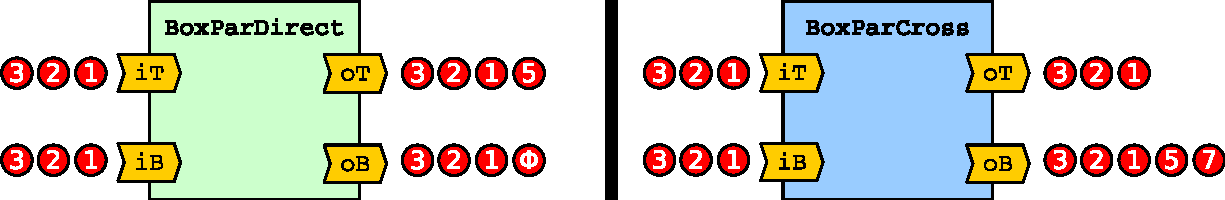
\includegraphics[width=0.8\linewidth]{graphics/connectivityTokens.pdf}
    \captionof{figure}{
      Bla Bla \\ 
      As can be seen
    }
    \label{fig:BoxTopTokens}
  \end{minipage}

\end{table*}
